% Sample file for AES paper
\documentclass[]{interact}
\usepackage[caption=false]{subfig}
\usepackage{epstopdf}
\usepackage[natbibapa,nodoi]{apacite}
\setlength\bibhang{12pt}
\renewcommand\bibliographytypesize{\fontsize{10}{12}\selectfont}
\usepackage[bookmarksnumbered,colorlinks,bookmarks,citecolor=blue,linkcolor=blue,urlcolor=blue,breaklinks,linktocpage]{hyperref}
\usepackage{xcolor}
\usepackage{listings}
\lstset{language=C++, showstringspaces=false, upquote=true, morekeywords={constexpr}, 
basicstyle=\ttfamily\small,
keywordstyle=\color{violet}\ttfamily,
 stringstyle=\color{red}\ttfamily,
 commentstyle=\color{green}\ttfamily,
}
\usepackage{amsmath} %maths
%\usepackage{geometry}                % See geometry.pdf to learn the layout options. There are lots.
%\geometry{letterpaper}                   % ... or a4paper or a5paper or ... 
%\geometry{landscape}                % Activate for for rotated page geometry
%\usepackage[parfill]{parskip}    % Activate to begin paragraphs with an empty line rather than an indent
\usepackage{graphicx}
\usepackage{url}


\usepackage{amssymb}
\usepackage{epstopdf}
\DeclareGraphicsRule{.tif}{png}{.png}{`convert #1 `dirname #1`/`basename #1 .tif`.png}


% Metadata Information
%\jyear{2010}
%\jmonth{October}
%\jvol{1}
%\jnum{1}
%

\begin{document}

% Page heads
\markboth{Anonymous}{}
%\markboth{Lazzarini and Timoney}{}

% Title portion
\title{A Theory of Higher-Order Frequency Modulation Synthesis}


%Author Info.
\author{
%\name{Anonymous}
%\name{Victor Lazzarini\thanks{email: Victor.Lazzarini@mu.ie}  
%and  Joseph Timoney\thanks{email: Joseph.Timoney@mu.ie}}
%\affil{Maynooth University, \\ Maynooth, Ireland}
}

\maketitle
%Abstract
\begin{abstract}
Frequency modulation (FM) and phase modulation (PM) are well-known synthesis methods, which have been deployed widely in musical instruments. In this article, we analyse the design of stacked FM synthesis and using a direct comparison with PM, we put forward a solution for the direct application of FM in higher-order modulation arrangements. We begin by reviewing the theory of first-order FM, contrasting it to PM. We then discuss the problems of extending first-order FM by
simply applying the modulation to the frequency, which may result in carrier drift caused by the
presence of DC in the modulating signal. We proceed to develop a formulation of second-order FM which is equivalent to the issue-free PM synthesis, and present an expression for the evaluation of the second-order FM spectrum. By virtue of the application of amplitude modulation concurrently with frequency modulation, we are able to eliminate the DC component and thus any carrier drift caused by it. These principles are then extended to higher-order topologies, 
where we note that in the general case, the modulation signal at each level is amplitude modulated by its own FM input. From this, we are able to advance the concept of an FM operator, analogous to the one used in PM instrument design. From this we demonstrate that feedback FM is also a practical possibility. Finally, moving from continuous to discrete time, we develop a reference C++ implementation for computer music applications, and discuss issues relating to digital implementations.
\end{abstract}

\begin{keywords}
sound synthesis; non-linear distortion; frequency modulation; phase modulation; feedback;
\end{keywords}

\section{Introduction}

Linear frequency modulation (FM) as a sound synthesis technique has had a long history of development, first explored by James Tenney, followed by
Jean-Claude Risset and John Chowning~\citep{Lazzarini2023}. It was given a theoretical treatment by \cite{ChowningFM}, where he demonstrated it could provide an economical method of producing dynamic spectra with both harmonic and inharmonic partials. FM was also shown to generate sounds previously only possible with the more computationally expensive means of additive synthesis. Through the similar, but more flexible form of phase modulation (PM), which was the actual object of analysis in Chowning's paper, the method was implemented in a very successful range of digital synthesisers, first by Yamaha~\citep{FMTheory}, then by other vendors. In this form it was expanded to support higher-order (or stacked) as well as feedback modulation. Both extensions can be characterised as forms of complex (as in \emph{multi-component}) PM. 

The mathematical formulation of FM and PM is generally accepted to stem from the early studies in radio frequency broadcasting~\citep{Bloch, Corrington}, but in fact its roots extend further back to John Bernoulli in 1694 \citep[p.1]{Watson}. The concept of an instantaneous frequency, as the time derivative of the phase angle, was first introduced in order to support the development of 
such modulation theory~\citep{Carlson}, and since \cite{Gabor} it has become a cornerstone of modern spectral audio theory \citep{Lazzarini2021}. In these early papers, the exact distinction between the two forms of modulation was not a concern for the authors, as the principles being developed could be implemented with either one of the methods. However, it is important to note that most of the mathematics underpinning these ideas, arising from the theory of Bessel coefficients, applies first and foremost to PM and only in a second instance to FM, as we will show in this paper. 

The subject of PM has been studied extensively since Chowning's original paper, in many cases under the misleading name of FM. A review article by~\cite{MoorerIEEE} showed that PM is in fact a particular instance of a wider class of nonlinear techniques, which may described by closed-form summation formulae. Such methods also include waveshaping~\citep{LeBrunWaveshaping}, 
asymmetric PM~\citep{palamin1988a}, phase distortion~\citep{LazzariniPD}, and different forms of formant synthesis~\citep{Lazzarini2017}. More widely, we have also seen the theory of FM/PM appear in the studies of rhythmic modulation \citep{Waadeland}, in the modelling of instrumental tones \citep{Horner1998,Horner1997,Horner1996} and within a differentiable digital signal processing scheme~\citep{DDX7}. 
Recently, we have had the development of adaptive techniques, such as adFM~\citep{LazzariniADFM}, which allows PM of arbitrary sources. The case of modified FM synthesis is also worthy of note, producing yet another variant of PM based on purely imaginary modulation indices~\citep{Lazzarini2010theory}. In addition to these methods, we have seen the introduction of the concept of Loopback FM~\citep{Smyth, Loopback}. The question of taming exponential FM~\citep{HutchinsXFM} in analogue and digital synthesis applications has also been the object of further studies~\citep{TimoneyEFM,Nielsen}. A survey of the state of the art of non-linear distortion synthesis techniques is found in Lazzarini~(\citeyear[chap.8]{Lazzarini2021}).

In this paper, we first clarify the differences between FM and PM, making sure that the definitions of the two techniques are well established. Then we will proceed to discuss the question of higher-order modulation, which is realised by the use of a stack of modulators. This is a technique that is well understood as far as a PM implementation is concerned, but has not yet received a treatment in FM terms. We begin by focusing on the specific case of second-order FM, for which an equivalent PM expression is derived. From this, we have both an implementation recipe in the form of a synthesis flowchart, and a means of deriving the resulting spectrum. Higher-order FM is then shown to be a generalisation of this particular case, with a practical implementation
through the concept of FM operators (analogous to the well-known PM operators described by \cite{FMTheory}). This also allows the implementation of a the special case of feedback, where the operator signal is used as a source for FM of itself. To complement, we put forward a reference implementation in C++ to illustrate the principles presented earlier on and discuss issues arising in digital applications.

Our motivation for this work is to put forward a well-defined theory of higher-order frequency modulation that is relevant to electronic and computer music applications, both digital and analogue. While PM has been the method of choice for the majority of implementations in the digital domain, it is the case that in some situations it is not possible or convenient to modulate the phase of a signal. In these cases, if frequency is available as a modulation parameter, then it would be useful to understand how this modulation can be extended to high orders. However, we will not be arguing that FM presents any advantages to PM in stacked or feedback arrangements in the typical computer music platforms where both can be subject to modulation. Maybe the ubiquitousness of PM has prevented a theory of high-order FM from being developed earlier on. It is also the case that while stacked PM is widely used, a derivation of its spectrum has not yet been put forward in the literature. So it is also our hope that this article may be helpful to fill some of the gaps of an otherwise well developed field of study.

We have found that even though the subject of FM/PM has been covered from many perspectives, there still remains a lot of confusion in the literature regarding the differences between these two methods. To the best of our knowledge, \cite{Moore:1990} was the first to discuss explicitly the subject in the computer music literature, but only as a footnote. More recently, \cite{Lazzarini2021}, \cite{LazzariniTimoney2021}, \cite{Nielsen}, \cite{Loopback}, and \cite{Hsu} have all provided, independently and from different angles, a more complete theoretical and practical treatment of the subject. In this paper we also aim to add to this body of knowledge. While FM/PM may be thought of as nearly equivalent in terms of simple first-order topologies, this may not be the case when higher-order modulation, as well as feedback, is employed. We will proceed by examining the subject from a practical standpoint first, then introduce the theory supported by three forms of illustration: algebra, graphics (plots/flowcharts), and later on, program code. This should allow readers to approach the subject using one or more of the representations they are familiar with. In the interest of open science, all scripts employed to generate graphical plots as well as programming examples are shared via an online repository (see link in Sec.~\ref{sec:conclusions}).

\section{Frequency Modulation}
FM synthesis is fairly straightforward to implement. In its most general form, a signal is used to control the frequency of an oscillator, producing an output with many partials. The frequency control may be exponential or linear. In this work, we concentrate on the latter form of FM. The technique has been described in terms of a fast linear \emph{vibrato}, which employs modulation frequencies within the audio range ($> 20$ Hz).  Audio rate FM synthesis was first explored in the early 1960s by Tenney~\citep{Tenney1964}, and the earliest extant code fragment implementing it in a digital environment is from 1968, by Risset~\citep{Lazzarini2023}.

We can take this intuitive description as our starting point. Vibrato has two fundamental parameters: rate and width. The latter is determined by the amplitude of the modulating signal and the former by its frequency. In the case of linear vibrato, we can define the width as the maximum absolute deviation from a centre frequency. While at sub-audio rates the result of vibrato is a certain fluctuation of pitch, as the modulation frequency and width increases the carrier output signal ceases to be perceived as a pure sinusoid and becomes a waveform whose spectrum features a number of partials. It is necessary that enough modulation is applied, making the oscillator instantaneous frequency negative at times, depending on the parameters employed.

We can represent a sinusoidal FM carrier signal $c(t)$ using the following expression,

\begin{equation}\label{eq:fm}
c(t) = \cos\left(2\pi \int_{0}^{t} f_c + m(x) dx \right).
\end{equation}

To facilitate the discussion, we can set the modulator to $m(t) = d \cos(2\pi f_m t)$, a sinusoid with amplitude
$d$ and frequency $f_m$. We then have a modulation frequency $f_m$ and a carrier frequency deviation $d$,
along with the carrier frequency $f_c$, as the main parameters of FM. As noted earlier, depending on the values of $d$ and $f_c$,
the instantaneous frequency of the signal becomes negative, so we require oscillators that can respond to this. 
Finally, we should stress that this is the definition of \emph{linear} frequency modulation, as opposed to \emph{exponential}, which involves the scaling of the pitch of an oscillator where the instantaneous frequency is strictly non-negative.

\section{Phase Modulation}

To formulate an equivalent expression for PM, we can first rewrite Eq.~\ref{eq:fm} as 

\begin{equation}\label{eq:pm}
c(t) = \cos(\phi(t)),
\end{equation}

\noindent that is, using a time-varying phase signal $\phi(t)$ to drive an oscillator.
Now we can put this function in terms of sinusoidal phase modulation (PM),

\begin{equation}\label{eq:pmod}
\phi(t) =  2\pi f_c t  + z \sin(2\pi f_m t).
\end{equation}

The advantage of the PM representation is twofold. First, we 
have a measure of the amount of modulation, $z$, that, as we can demonstrate, does not depend on the
modulation frequency; and, second, we can take advantage of the Jacobi-Anger 
expansion~\citep[p.22]{Watson}, to determine the spectrum of the phase modulation signal,

\begin{equation}\label{eq:jacobi-anger}
\begin{split}
e^{\pm jz\sin(\theta)}  &= J_{0}(z) + 2 \sum_{n=1}^{\infty} J_{2n}(z)\cos\left(2n\theta\right) \\
& \pm 2j \sum_{n=0}^{\infty} J_{2n+1}(z)\sin\left([2n+1]\theta\right),
\end{split} 
\end{equation}

\noindent where $J_n(z)$ is the Bessel coefficient of order $n$. From this equation and its application
to Eq.~\ref{eq:pmod}, we can observe that $z$ is directly involved in determining the amount of energy spread from
the carrier partial to the various sidebands. Finally, it should be noted that an ancillary advantage of PM over
FM in digital applications is that it is more resilient to numerical errors, as will become clear in Section~\ref{sec:digital}.

\subsection{Equivalence to FM}\label{sec:fmvpm}

In order to connect this to the FM expression of Eq.~\ref{eq:fm}, we can find 
the corresponding instantaneous carrier frequency as the derivative of the phase
signal $\phi(t)$ in Eq.~\ref{eq:pmod}~\citep[p.318]{Moore:1990},

\begin{equation}
\dot{\phi}(t) = 2\pi \left [f_c  + z f_m \cos(2\pi f_m t) \right]. 
\end{equation}

The quantity $z f_m$, the product of the modulation frequency and the phase modulation amount
is equivalent to the frequency deviation $d$ employed in the FM signal. We use the term 
\emph{modulation index} to characterise $z$,

\begin{equation}\label{eq:deviation_fm}
z =  \frac d {f_m}.
\end{equation}

As shown before, the modulation index determines the spread of the resulting FM/PM spectrum.
From Eq.~\ref{eq:jacobi-anger}, we can derive

\begin{equation}\label{eq:pm_synthesis}
\cos\left(\omega + \frac d {f_m} \sin(\theta)\right) = \sum_{n=-\infty}^{\infty} J_n\left(\frac d {f_m}\right)\cos\left(\omega + n\theta\right),
\end{equation}

\noindent with $\omega = 2\pi f_c t$, $\theta = 2\pi f_m t$, and using the identity $J_{-n}(z) = (-1)^n J_n(z)$. 
This demonstrates that the amplitude of the frequency modulator, $d$, cannot alone be used as
a measure of the amount of modulation applied to the carrier signal. On the other hand,
as we noted earlier, the amplitude of the phase modulator, $z$, can be applied directly to determine the output spectrum.
This is the sense of the statement that the theory of Bessel functions applies to FM only in a second instance, once
we have translated it into an equivalent PM form.

We can see that the FM spectrum of Eq.~\ref{eq:fm} (and its corresponding PM expression, Eq.~\ref{eq:pm}) is composed of partials at $f_c \pm n f_m$ Hz, which are scaled by the corresponding Bessel function coefficient $J_n(z)$. We now have a mechanism to 
represent FM in terms of PM, which provides a clear route for analysis. The two
methods have distinct implementations, a comparison between the FM and PM flowcharts 
is shown in Fig.~\ref{fig:fmpm}.

\begin{figure}[htp]
\begin{center}
\includegraphics[width=.5\columnwidth]{fmpm.png}
\caption{Flowcharts for PM (left) and FM (right).}
\label{fig:fmpm}
\end{center}
\end{figure} 

\section{Second-Order FM}\label{sec:theory}

 The case of Eq.~\ref{eq:fm} is that of first-order modulation,
consisting of one modulator and one carrier oscillator. We now consider the arrangement whereby this is increased
to a second order, that is, where two modulation stages are present. An FM carrier wave is then 
used as a modulator to a subsequent carrier oscillator. This can then be extended to higher orders
where the output signal is the result of several stages of modulation. It has been claimed in the literature
that, unlike PM, FM synthesis cannot be implemented in higher-order topologies~\citep{PinkstonFM}, but
as we will demonstrate, that is the not the case. 

Many of the difficulties arise from a simplistic approach
to the implementation of FM synthesis that does not take into account the differences we have discussed
in section \ref{sec:fmvpm}. It is also the case that some synthesisers implement direct forms of FM allowing 
the possibility of higher-order modulation topologies (and even feedback) (see for instance \cite{Summit}). 
However, there are deficiencies in these designs, which we address in this paper. Our motivation here is
to have an equivalent form of higher-order FM that produces results similar to PM. 

\subsection{Analysis}

We first need to consider the amount of modulation required at each stage. A na\"{i}ve approach,
following directly from the single-level example, would lead us to apply simply the product of an index of
modulation $z_n$ and modulation frequency $f_{m_n}$ to determine the frequency deviation at each stage $n+1$. 
If we aim to achieve a spectrum similar to PM, not only this is incorrect from a mathematical point of view, but we 
may also observe some problematic results. 

As an example of the pitfalls involved in a simplistic approach, we may consider the case of a particular second-order modulation stack, such as may be found for instance in the implementation of the Summit synthesizer \citep{Summit}. In this we have a first order modulator with frequency $
f_{m_0}$, modulating a second-order modulator with frequency $f_{m_1}$, which then modulates 
a carrier oscillator with frequency $f_{c}$, where we set $f_{m_0} = f_{m_1} = f_c$. The FM expression is thus

\begin{equation} \label{eq:naive1}
a\cos\left(2 \pi \int_0^t f_c + d_1 m_1(x) dx\right),
\end{equation}

\noindent and the carrier is modulated by the signal $m_1(t)$ from the first order stage,

\begin{equation} \label{eq:naive2}
m_1(t) = \cos\left(2\pi \int_0^t f_{m_1} + d_0 m_0(x) dx\right),
\end{equation}

\noindent with $m_0(t) = \cos(2\pi f_{m_0} t)$. This na\"{i}ve FM stack is depicted in
Fig.~\ref{fig:stacked_naive}.

\begin{figure}[htp]
\begin{center}
\includegraphics[width=.5\columnwidth]{naivestack.png}
\caption{Na\"{i}ve second-order FM stack.}
\label{fig:stacked_naive}
\end{center}
\end{figure} 

We know from Eq.~\ref{eq:pm_synthesis} that the resulting spectrum of $m_1(t)$
will contain partials at $f_{m_1} \pm nf_{m_0}$. For $n = -1$, we have a component
at $f_{m_1} - f_{m_0} = 0$ Hz (DC), whose amplitude is given by $-J_{1}\left(d_0/f_{m_0}\right)$. When this modulation signal is then applied to the frequency $f_c$ of the carrier oscillator at the next stage, the DC term is simply added as an offset to $f_c$. We can see now that this will result in a shift of the carrier frequency that is proportional to $-d_1J_{1}(d_0/f_{m_0})$. Changes in the modulation index at the top level will then imply a carrier drift. Worse, a change in $d_1$ will also cause $f_c$ to be scaled further.

Such an effect ties in timbral changes with partial glides, which in most cases makes it difficult to implement dynamic spectra. Generally with standard FM/PM we should not expect any shift in partial frequencies as we increase or decrease the amount of modulation. There is a separation between the setting of partial frequencies, which is dependent on the ratios of modulators and carrier, and the partial
amplitudes, given by the index of modulation. In Figures~\ref{fig:naive0} and ~\ref{fig:naive1}, we can see the result of applying a change of index of modulation to the $m_0(t)$ and $m_1(t)$ signals, respectively, using a linear envelope from 0 to 2. In these spectrograms, it is possible to see how the change in the amount of modulation at both levels has an effect on the partial frequencies make them glide divergently as the carrier frequency drifts.

\begin{figure}[htp]
\begin{center}
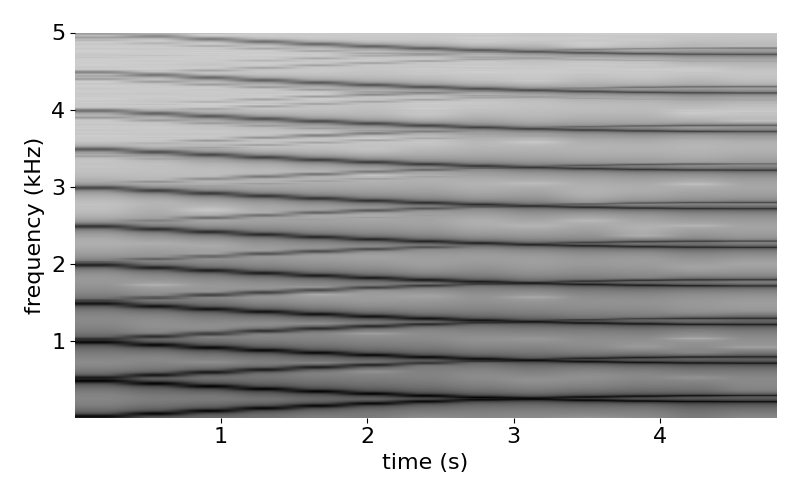
\includegraphics[width=0.9\columnwidth]{naive0.png}
\caption{Spectrogram of na\"{i}ve second-order stacked FM output, with $f_{m_0} = f_{m_1} = f_c = 500$ Hz, $d_1 = f_m0$, applying a linear envelope applied to $d_0$, $0 \leq d_0 < 2f_{m_0}$.}
\label{fig:naive0}
\end{center}
\end{figure} 

\begin{figure}[htp]
\begin{center}
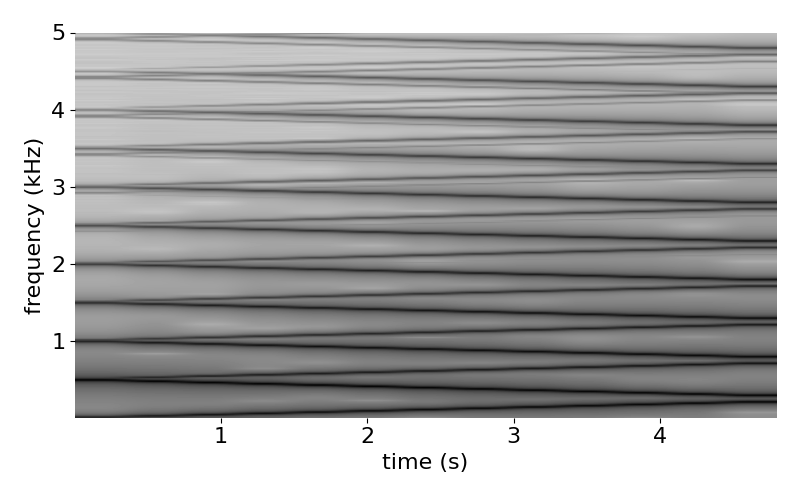
\includegraphics[width=0.9\columnwidth]{naive.png}
\caption{Spectrogram of na\"{i}ve second-order stacked FM output, with $f_{m_0} = f_{m_1} = f_c = 500$ Hz, $d_0 = f_m0$, applying a linear envelope applied to $d_1$, $0 \leq d_1 < 2f_{m_1}$.}
\label{fig:naive1}
\end{center}
\end{figure} 

It is of course possible to select modulation frequency ratios that do not result in the modulation signals producing any DC components, and also to produce spectra with a strict $-\pi/2$ (sine) phase at 0 Hz. However these solutions are not general enough to support a theory of higher-order FM synthesis. 

Note that such issues do not occur in PM, since any DC offset is translated as a phase shift,
rather than a carrier frequency drift. For this reason, as we have already indicated, 
it is generally much more flexible to adopt PM as a general method for higher-order modulation. 
We should conclude that a satisfactory solution could be developed by deriving a PM-equivalent
form for second-order FM. Using the principles developed earlier, we observe that the integration involved in FM synthesis (cf Eq.~\ref{eq:fm}) requires that some form of periodic time-varying deviation is applied to the signal. Since the instantaneous frequency of an FM signal is time-varying, it implies the presence of an amplitude modulation term following integration. We should
conclude that we need to apply both FM and AM concurrently in the modulation stack.

To demonstrate this, let's review Eqs.~\ref{eq:naive1} and~\ref{eq:naive2}. We are trying to generate a modulation signal $m_1(t)$ whose frequency $f_{m_1}$ is itself modulated by a sinusoidal signal $m_0(t)$, whose frequency is $f_{m_0}$. If we want to apply an index of modulation $z_0$, then according to Eq.~\ref{eq:deviation_fm}, we need to set the $m_0(t)$ signal amplitude $d_0$ to $z_0 f_{m_0}$. The time-varying frequency $f(t)$ of the modulator $m_1(t)$ is then 

\begin{equation}
f(t)  = f_{m_1} + z_{0} f_{m_0} m_0(t),
 \end{equation}

Therefore, also according to Eq.~\ref{eq:deviation_fm}, 
we need to employ the following time-varying deviation, 
with an appropriate value of $z_1$,

\begin{equation} \label{eq:deviation_stack}
d_1(t) = z_1 f(t) = z_1 [f_{m_1} + z_{0} f_{m_0} m_0(t)],
\end{equation}

\noindent in order to produce the frequency modulation signal $d_1(t)m_1(t)$, which
we will use to modulate the frequency of the carrier oscillator. With this, we
have produced a PM-equivalent modulation signal.

\subsection{Synthesis}

We can now apply these principles to the typical case of a second-order FM synthesis arrangement using two sine wave oscillators. The solution developed for this case can then be expanded to provide methods for higher-order modulation topologies. Using the notions developed above, we can now describe the correct form of second-order FM as

\begin{equation} \label{eq:fmstacked}
\begin{split}
&m_0(t) =  \cos(2\pi f_{m_0} t)\\
&m_1(t) = \cos\left(  2\pi\int_{0}^{t} f_{m_1} + z_0  f_{m_0} m_0(x)dx\right) \\
&c(t) =  \cos\left(2\pi \int_{0}^{t} f_c + z_1 [f_{m_1} + z_0 f_{m_0} m_0(x)] m_1(x) dx \right). \\
\end{split}
\end{equation}

From these equations, we can see in this equation that the modulator at level 1, $m_1(t)$, is amplitude modulated by its own modulator, $m_0(t)$, when applied to the carrier frequency. We will be able to build on this principle later on as we extend the method to higher orders.
We can now demonstrate how these equations are equivalent to the typical form
of second-order PM. To do this, we begin by reworking the first-order modulation 
as a PM expression,

\begin{equation}\label{eq:fm+pm}
\begin{split}
&m_0(t) = \sin(2\pi f_{m_0} t)\\
&\phi(t) = \cos(2\pi f_{m_1} t + z_0 m_0(t)) \\
&c(t) =  \cos\left(2\pi \int_{0}^{t} f_c + z_1 [f_{m_1} + z_0 f_{m_0}\cos(2\pi f_{m_0} x)] \phi(x) dx\right). \\
\end{split}
\end{equation}

The next step is to replace $\phi(.)$  in the carrier signal 
equation,

\begin{equation}
\begin{split}
c(t) = \cos\Bigg(2\pi \int_{0}^{t} &f_c  + z_1 [f_{m_1} + z_0 f_{m_0} \cos(2\pi f_{m_0}x)] \times\Bigg.\\
&\Bigg. \cos\left(2\pi f_{m_1} x + z_0\sin(2\pi f_{m_0}x)\right) dx\Bigg),
\end{split}
\end{equation}

\noindent which translates as the following expression describing second-order PM

\begin{equation}\label{eq:pm_stack}
c(t) = \cos\left(2\pi f_c t + z_1\sin\left(2\pi f_{m_1} t + z_0\sin(2\pi f_{m_0} t)\right) \right).
\end{equation}

The equivalent FM topology (Eq.~\ref{eq:fmstacked}) can be implemented 
using the flowchart shown in Fig.~\ref{fig:stacked}. In this, we see that in order to 
implement stacked FM we need to take into account the amplitude modulation effects that arise
from employing a modulated input, as per Eq.~\ref{eq:deviation_stack}.

\begin{figure}[htp]
\begin{center}

\includegraphics[width=.3\columnwidth]{stacked.png}
\caption{Second-order FM flowchart.}
\label{fig:stacked}
\end{center}
\end{figure} 

Continuous-time waveforms and their spectra produced by second-order FM and PM are shown
to be exactly equivalent in Fig.~\ref{fig:fm-pm}. These signals were produced using the approach
described by Eq.~\ref{eq:fmstacked} and Fig~\ref{fig:stacked}, in the case of FM, and the
corresponding PM expression given in Eq.~\ref{eq:pm_stack}. We have now demonstrated that it 
is indeed possible to use a second-order FM topology to produce a spectrum that is similar 
to second-order PM.  

\begin{figure}[htp]
\begin{center}
\includegraphics[width=.75\columnwidth]{../fm-pm.png}
\caption{Second-order FM (left) and PM (right) waveforms and normalised spectra from Eq.~\ref{eq:fmstacked} (Fig.~\ref{fig:stacked}) and Eq.~\ref{eq:pm_stack}, respectively, with $f_c = f_{m_0} = f_{m_1} = 500$ Hz, $z_0=3$, and $z_1=2$}.
\label{fig:fm-pm}
\end{center}
\end{figure} 

\subsection{Spectrum}

With its equivalent PM form, we can now derive an expression for the second-order FM spectrum. Using
Eq.~\ref{eq:jacobi-anger} we rewrite Eq.~\ref{eq:pm_stack} as

\begin{equation}
c(t) =  \cos\left( 2\pi f_c t + z_1 \sum_{n=-\infty}^{\infty} J_n(z_0)\sin\left(2\pi [f_{m_1}  + n f_{m_0}] t\right)\right).
\end{equation}

From this equation we can now use a derivation of the spectrum of complex PM~\citep{LeBrunFM}. In order to make this 
more meaningful, we assume that the first-order output signal spectrum contains only $K_0$ sidebands 
with significant energy (rather than the theoretically non-bandlimited spectrum). The expansion of
second-order FM synthesis equation can then be given as 

\begin{equation}\label{spectrumeq}
\begin{split}
\sum_{\eta_{-K_0}=-\infty}^{\infty} \ldots \sum_{\eta_{K_0}=-\infty}^{\infty}
&\prod_{k_0=-K_0}^{K_0} J_{\eta_{k_0}}\left(z_1 J_{k_0}(z_0)\right)\\
&\cos\left(2 \pi [f_c  + \sum_{k_0=-K_0}^{K_0} \eta_{k_0}(f_{m_1} + k_0 f_{m_0})] t \right).
\end{split}
\end{equation}

The value of $K_0$ is dependent on the first-order modulation index $z_0$ and will increase as more
modulation is inserted into the signal. We should note that Eq.~\ref{spectrumeq} is reduced to Eq.~\ref{eq:pm_synthesis} if $z_0 = 0$,

\begin{equation}
\sum_{\eta_0=-\infty}^{\infty} J_{\eta_0}\left(z_1\right) \cos\left(2 \pi [f_c  + \eta_0 f_{m_1}] t \right),
\end{equation}

\noindent since in this case there is no modulation at the first-order stage, $K_0=0$, and $J_0(0) = 1$. 
From \cite{Lazzarini2021}, a reasonable estimate for this can be found as $K_0 \approx z_0 + l$, $z_0 > 1$, with $2 \lessapprox  l \lessapprox  3$. Using a similar approximation for the number of second-order sidebands based on $z_1$, the case of Fig~\ref{fig:fm-pm} is thus given by

\begin{equation}\label{spectrumeq}
\begin{split}
\sum_{\eta_{-5}=-4}^{4} \ldots \sum_{\eta_{5}=-4}^{4} &\prod_{k_0=-5}^{5} J_{\eta_{k_0}}\left(2 J_{k_0}(3)\right)\\
&\cos\left(2 \pi [f_0  + \sum_{k_0=-5}^{5} \eta_{k_0} f_0(k_0+1)] t \right),
\end{split}
\end{equation}

\noindent with $f_0 = 500$ Hz. We can observe in Fig.~\ref{fig:fm-pm} that this second-order FM/PM spectrum 
extends to a 15500 Hz partial at -90 dB, and the above expression with $K=5$ describes the spectrum up to 
12500 Hz ($\sim$70 dB below the loudest harmonic).

This derivation of the second-order FM spectrum brings to the fore two important aspects.
Firstly, we should note that, as indicated by Eq.~\ref{spectrumeq}, the resulting spectrum may be very
complex and difficult to predict if $z_0$ and $z_1$ are large. In that case there will be many
sidebands with frequencies $f_c \pm n_{k_0} f_{m_1} \pm k_0 \eta_{k_0} f_{m_0}$ with significant intensity interacting with each other. Secondly, we may reduce second-order FM as a first-order case employing a complex modulator, but
with the advantage that we can change the spectrum of the modulating wave via a single
parameter, $z_0$. Such arrangement generally calls for small modulation indices. This is 
in fact a good reason for employing second (or higher)-order modulation topologies;
we find that smoother FM spectral changes are better achieved with indices that range from 
0 to a small positive value~\citep{Lazzarini2021}. As in the case of a complex modulating wave,
it is possible to achieve partial-rich spectra with much more reduced modulation compared
to simple first-order sinusoidal modulation. 

\section{Higher-order Modulation}
The method developed here for second-order modulation may be expanded to higher-order arrangements,
as needed. After proving the equivalence of Eq~\ref{eq:fmstacked} to the PM expression given by
Eq~\ref{eq:pm_stack}, we can now extend it to an arbitrarily high order. A stack of modulators of
order $n$ is thus given as

\begin{equation}\label{eq:high-order}
\begin{split}
&m_0(t) =  \cos(2\pi f_{m_0} t)\\
&m_1(t) = \cos\left(  2\pi\int_{0}^{t} f_{m_1} + z_0  f_{m_0} m_0(x)dx\right) \\
&m_2(t) =  \cos\left(2\pi \int_{0}^{t} f_{m_2} + z_1 [f_{m_1} + z_0 f_{m_0} m_0(x)] m_1(x) dx \right) \\
&\ldots \\
&m_{n-1}(t) =  \cos\left(2\pi \int_{0}^{t} f_{m_{n-1}} + z_{n-2} [f_{m_{n-2}} + z_{n-3} f_{m_{n-3}} m_{n-3}(x)] m_{n-2}(x) dx \right) \\
&c(t) =  \cos\left(2\pi \int_{0}^{t} c + z_{n-1} [f_{m_{n-1}} + z_{n-2}f_{m_{n-2}} m_{n-2}(x)] m_{n-1}(x) dx \right). \\
\end{split}
\end{equation}

The modulation signal at each level $m$, $m > 0$, is amplitude modulated by its own FM input. 
We observe that in general if a signal whose instantaneous frequency changes significantly 
over time is used for FM, then we will need to account for this in the integration. 
From another perspective, we can also observe that through amplitude modulation, we are able to suppress 
the DC signals responsible for any carrier drift. 

The spectrum of stacked FM at order $n$ is duly obtained by extending Eq.~\ref{spectrumeq} as

\begin{equation}\label{eq:high-order-spec}
\begin{split}
\left[\sum_{\eta_{-K_0}=-\infty}^{\infty} \ldots \sum_{\eta_{K_0}=-\infty}^{\infty}\right] &\ldots \left[\sum_{\eta_{-K_{n-2}}=-\infty}^{\infty} \ldots \sum_{\eta_{K_{n-2}}=-\infty}^{\infty}\right]\\
\left[\prod_{k_0=-K_0}^{K_0} J_{\eta_{k_0}}\left(z_1 J_{k_0}(z_0)\right)\right] &\ldots 
\left[\prod_{k_{n-2}=-K_{n-2}}^{K_{n-2}} J_{\eta_{k_{n-2}}}\left(z_{n-1} J_{k_{n-2}}(z_{n-2})\right)\right]  \\
\cos\Bigg(2 \pi \bigg[f_c  + &\sum_{k_0=-K_0}^{K_0} \eta_{k_0}(f_{m_1} + k_0 f_{m_0}) + ... + \\
& \sum_{k_{n-2}=-K_{n-2}}^{K_{n-2}} \eta_{k_{n-2}}(f_{m_{n-1}} + k_{n-2} f_{m_{n-2}})\bigg] t \Bigg).
\end{split}
\end{equation}

\noindent with same approximations $K_m \approx z_m + l$ at each modulation level $m$. As can be seen, the complexity of the spectrum can increase significantly depending on the order, the modulation frequencies and indices.

\subsection{Operators}

In order to facilitate the design of instruments using higher-order FM topologies, we
can take advantage of the concept of an \emph{operator}. At its simplest, this is a sinusoidal
oscillator whose frequency can be modulated by another. The principle of an operator is very 
common in PM synthesis \citep{FMTheory}, and it may also include an envelope to 
allow for dynamic spectra as well as amplitude shaping. In PM, an operator is characterised
by a phase modulation input, plus amplitude and frequency parameters, and a single output. Operators 
can be connected in series (stacked), or in parallel. For FM, we can develop a similar black-box 
approach.

To design an operator for FM, we need to take account of our analysis in 
Section \ref{sec:theory}. We may note that within a stack, the top oscillator takes in
a modulation frequency and a modulation index, producing a modulation signal. Subsequent
oscillators take in a modulation signal in addition to the frequency and index. At the bottom of 
the stack, an oscillator produces the output signal, and it takes an amplitude instead of a modulation 
index. As in PM, the operator takes three inputs (index/amplitude and frequency scalars 
plus modulation signal). The specification requires that we make no distinction between amplitude
and index. For this to be practical, unlike in the PM case, we would then need to distinguish between 
audio and modulation outputs. For this reason, a freely-stackable FM operator requires 
two separate outputs. Envelopes may be added to shape the scalar input parameters. In pseudocode, 
the simplest design would be

\begin{lstlisting}
audio,modulation = operator(amplitude,frequency,modulation)
\end{lstlisting}

With this, the second-order stack discussed earlier would be defined as

\begin{lstlisting}
audio,mod0 = operator(index0,fm0,0)
audio,mod1 = operator(index1,fm1,mod0)
audio,mod = operator(amp,fc,mod1)
\end{lstlisting}

The implementation of the operator black box is shown in Fig~\ref{fig:operator}, together with
an arrangement of three operators in a second-order modulation topology equivalent to that
of Fig~\ref{fig:stacked}. 

\begin{figure}[htp]
\begin{center}
\includegraphics[width=.5\columnwidth]{operator.png}
\caption{FM operator (left) and second-order modulation arrangement (right). The \emph{a} and \emph{f}
parameters represent the scalar index/amplitude and frequency.}
\label{fig:operator}
\end{center}
\end{figure} 

As can be seen, the actual signal flow is re-ordered somewhat with the
product being placed at the output of the oscillator. This way it is possible to use a single operator
be either a carrier or a modulator in any arrangement of any order. The topmost modulator will
always have no signal inputs and we only use the audio signal out of the carrier operator. Also
we should note that this allows us to tap anywhere into an FM topology to retrieve an audio
signal at that point. Dynamic spectra can be implemented by including envelopes to control
the \emph{a} and \emph{f} parameters in Fig~\ref{fig:stacked}.

\subsection{Feedback}

The operator as developed here opens up the possibility of implementing a feedback FM design, which 
is analogous to feedback PM as introduced by \cite{Tomisawa}. Confusingly, his technique 
has been called feedback FM in the literature, which only served to murky the waters. We should
continue to make the distinctions we made before between FM and PM, thus we will refer to Tomisawa's
method as feedback PM.

Feedback FM can be thought of as a form of high-order FM, where an infinite number of modulators are stacked, all with the same frequency. To construct this, we just need to apply the modulation recursively, as in

\begin{lstlisting}
audio,modulation = operator(amplitude,frequency,modulation),
\end{lstlisting}

\noindent which is depicted as a flowchart in Fig~\ref{fig:feedback}.

\begin{figure}[htp]
\begin{center}
\includegraphics[width=.5\columnwidth]{feedback.png}
\caption{FM operator with feedback (left) and its black-box representation (right).}
\label{fig:feedback}
\end{center}
\end{figure} 

For an operator with unity amplitude whose frequency is $f_0$, the feedback FM formula arising from 
its arrangement can then be put as

\begin{equation}
\omega(t) = \cos\left(2\pi \int_0^t [f_0 + \omega(x)]\omega(x) dx\right),
\end{equation}

\noindent which seems intractable at first. However, after \cite{Mitsuhashi}, we can determine 
a complex PM expression that is equivalent to it,

\begin{equation}
\omega(t) = \cos\left(2\pi f_0 t + 2 \sum_{n=1}^{\infty} \frac {J_{n}(n)} n \sin(2\pi n f_0 t)\right) 
\end{equation}

\noindent This corresponds to a cosine whose phase is modulated by a complex
waveform $m(t)$. A similar expression can also be used to 
describe the elliptic motion of a planet about the sun, as shown by 
Lagrange in 1770~\citep[p.6]{Watson}. From there we can derive the spectrum of feedback FM as 

\begin{equation}
\omega(t) = -\frac 1 2 + 2 \sum_{n=1}^{\infty} \frac{\dot{J}_n(n)} n  \cos(2\pi n f_0 t),
\end{equation}

\noindent with $2\dot{J}_n(n) = J_{n-1}(n) - J_{n+1}(n)$. It is interesting to note that in this
case, the spectral description is considerably more simplified and compact than in the
general case of higher-order FM as shown by Eq.~\ref{eq:high-order-spec}.

It is also noteworthy to contrast this with feedback PM \citep{Tomisawa}, defined by

\begin{equation}
\phi(t) = \sin\left(2\pi f_0 t + \phi(t)\right),
\end{equation}

\noindent which actually corresponds to $m(t)$~\citep[p.62]{Benson},

\begin{equation}
\phi(t) = 2 \sum_{n=1}^{\infty} \frac {J_{n}(n)} n \sin(2\pi n f_0 t).
\end{equation}

\noindent Since $2 \frac{J_{n}(n)} n \approx \frac 1 n$, this is very nearly a sawtooth wave.

The spectrum and waveform of feedback FM is shown on Fig.~\ref{fig:feedbackspec} 
alongside feedback PM. As we can see, if we exclude the negative DC term, 
the two spectra share many similarities, although the waveforms are different. This is mostly to do with different partial phases. While the feedback PM formula produces an odd waveform, therefore a purely imaginary spectrum, feedback FM results in an even waveform, featuring a purely real spectrum. This is due to the fact that sine wave modulators are guaranteed to produce only sine wave sidebands with a sine carrier and a strictly cosine wave spectrum with a cosine carrier (cf Lazzarini,~\citeyear[chap.8]{Lazzarini2021}). We also observe that the feedback FM spectral envelope has slightly more accentuated rolloff, defined
by a $\dot{J}_n(n)/J_{n}(n)$ factor for each harmonic $n$. 

\begin{figure}[htp]
\begin{center}
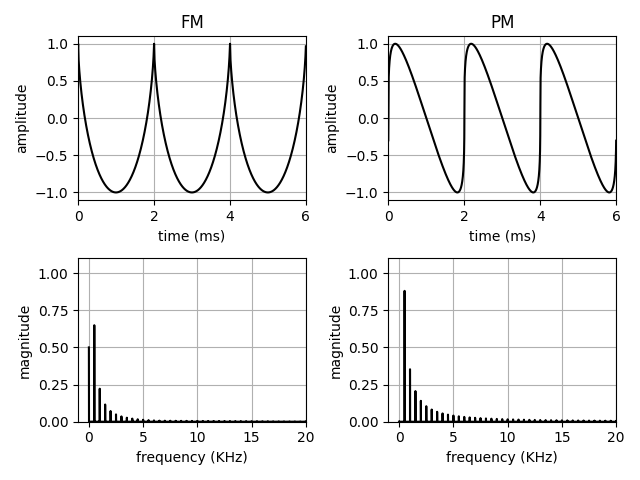
\includegraphics[width=.75\columnwidth]{feedback-sp.png}
\caption{Feedback FM (left) and PM (right) waveforms and spectra, with $f= 500$ Hz.}
\label{fig:feedbackspec}
\end{center}
\end{figure} 

Dynamic spectra in this arrangement is possible through applying an envelope to the amplitude $a$, $|a| \leq 1$, 
of the operator, resulting in

\begin{equation}
 -\frac {a^2} 2 + 2a \sum_{n=1}^{\infty} \frac{\dot{J}_n(an)} n  \cos(2\pi n f_0 t).
\end{equation}

\noindent As can be seen, $a$ has an effect on both amplitude and bandwidth, as the
feedback modulation increases at the same time as the operator output. If we want to decouple these,
it is possible to keep the operator amplitude at unity, and employ a separate gain $|g| \leq 1$  to 
control the feedback amount. The amplitude control can then be applied to the audio and modulator 
outputs. An operator including internal feedback with independent amplitude and bandwidth control is
shown in Fig.~\ref{fig:feedback-op}.

\begin{figure}[htp]
\begin{center}
\includegraphics[width=.5\columnwidth]{operator-fdb.png}
\caption{FM operator including an internal feedback path with independent control of amplitude ($a$) and feedback gain ($|g| \leq 1$) (left) 
and its black-box representation (right).}
\label{fig:feedback-op}
\end{center}
\end{figure} 

Finally, it is important to note the aforementioned technique of loopback FM introduced by \cite{Loopback}, which as opposed to
feedback FM does not intend to provide a feedback PM-analogous spectrum. Instead, it employs
the output of the oscillator directly to modulate its own frequency, with distinct spectral results.
This has received a thorough treatment by \cite{Hsu}, where it is contrasted to the standard
technique of feedback PM.

\section{Digital Implementation}\label{sec:digital}

Following the exposition of the theory in continuous time, we can now turn to look at the implementation of higher-order FM using digital oscillators. We first provide a reference implementation in C++ for an operator, together with a second-order example. This is followed by an analysis of issues arising in digital FM synthesis and practical mitigation methods.

\subsection{Reference Implementation in C++}

The following code provides a reference implementation of the FM synthesis
operator, including an internal feedback path, as depicted in Figs.~\ref{fig:operator} and~\ref{fig:feedback-op}:

\begin{lstlisting}
#include <vector>
#include <cmath>

template<typename S>
class Op {
  static constexpr long maxlen = 0x100000000; 
  const std::vector<double> &tab;  
  std::vector<S> out;
  std::vector<S> mod;
  S fdb;
  unsigned int fs;  
  unsigned int phs;
  unsigned int lobits;
  unsigned int fac;
  unsigned int lomask;
  double nfac;
  
  double lookup(S f){
    unsigned int ndx = phs >> lobits; 
    auto s = tab[ndx] +
      nfac*(phs & lomask)*(tab[ndx+1] - tab[ndx]); 
    phs += (int)(f*fac); 
    return s;
  }

  const std::vector<S> &process(S a,S fr,
                                const S* fm,S g){
    std::size_t n = 0;
    for(auto &o : out) {
      auto f = fr+fdb*g+(fm?fm[n]:0);
      auto s = lookup(f);
      mod[n++] = (S) ((fdb = s*f)*a);
      o = (S) (a*s);
    }
    return out;
  }

public:
  Op(const std::vector<double> &table, unsigned int sr, 
     std::size_t vsize) :
    tab(table),out(vsize),mod(vsize),fdb(0),fs(sr),
    phs(0),lobits(0),fac(maxlen/sr){
    for(unsigned long t = tab.size()-1; 
        (t & maxlen) == 0; t <<= 1) lobits += 1;
    lomask = (1 << lobits) - 1;
    nfac = 1./(lomask + 1);
  }

  unsigned int vsize(){return out.size();}
  unsigned int sr(){return fs;}
  const S *data(){return out.data();}
  
  const std::vector<S> &operator()(){return mod;}
  const std::vector<S> &operator()(S a,S fr,S g=0){
    return process(a,fr,nullptr,g);
  }
  const std::vector<S> &operator()(S a, S fr,
                                   const std::vector<S> &fm,
                                   S g = 0) {
    return process(a,fr,fm.data(),g);
  }
};
\end{lstlisting}

\noindent The table lookup oscillator in this implementation employs fixed-point phase computation, thus wavetables
are required to have a power-of-two plus one size (the extra point is used for linear interpolation). By employing 
a fixed-point function table and normalisation factor, the code could also be deployed in platforms with no 
floating-point support. 

Using instances of this class, we can implement various types of high-order FM synthesis topologies. For example, a 
second-order stacked FM arrangement, such as the one described in Fig.~\ref{fig:stacked}, can be 
modelled using the following code:

\begin{lstlisting}
const std::size_t def_vsize = 64;

template<typename S> class StackedFM {
  std::vector<double> table;
  Op<S> mod0; 
  Op<S> mod1;
  Op<S> car;
  
public:
  StackedFM(unsigned int fs, std::size_t vsize = def_vsize) :
    table(1025),mod0(table,fs,vsize),mod1(table,fs,vsize),
    car(table,fs,vsize) {
    std::size_t n = 0;
    for(auto &s : table)
      s = std::cos(twopi/(table.size()-1)*n++);
  };

  unsigned int vsize() { return car.vsize(); }
  unsigned int fs() { return car.sr();}
  const S *data() { return car.data(); }

  const std::vector<S> &operator()(float a,float fc,
                                   float fm0,float fm1,
				   float z0,float z1) {
    mod0(z0,fm0);
    mod1(z1,fm1,mod0());
    return car(a,fc,mod1());
  }
};
\end{lstlisting}

An object of this class can then be used to produce
an FM tone as shown by an example program fragment. 
It uses modulation frequencies set to $c = m_0 = m_1$ with separate
indices of modulation for first and second-order stages (\lstinline{z0}, \lstinline{z1}):

\begin{lstlisting}
StackedFM<float> fm(fs);

for(n = 0; n < fm.fs()*dur; n += fm.vsize()) {
 auto& sig = fm(amp,fr,fr,fr,z0,z1);
 for(auto s : sig)
   std::cout << s << std::endl;
}
\end{lstlisting}


\subsection{Issues}

We normally expect a digital implementation to produce a signal that is fairly faithful to the continuous-time equations, if enough
mathematical precision is employed. However, in practice we observe a certain amount of phase drift whenever 
an FM signal is generated using digital oscillators, due to errors associated with the use of a discrete-time 
integrator. As demonstrated by the reference code, the instantaneous phase of a digital oscillator is usually 
computed using an infinite impulse response filter defined by

\begin{equation}\label{eq:dinteg}
y(n) = x(n) + y(n-1), 
\end{equation}
\smallskip

\noindent to which a frequency signal, $x(n) = f(n)/f_s$, is applied (with $f_s$ denoting the sampling frequency). Defining the
digital integration filter (Eq.\ref{eq:dinteg}) as the operator integ$[.]$, the output of digital FM can be described by

\begin{equation}
\nu(n) = \cos\left(2\pi\:\textrm{integ}\left [\frac {f_{m_1} + z_0 f_{m_0} \cos\left(2\pi f_{m_0} \frac n {f_s}\right)} {f_s} \right] \right).
\end{equation}
\smallskip

The net effect of the integration error is to add an extra term to $\phi(t)$ in Eq.~\ref{eq:fm+pm}. If we set $t = n/f_s$,
we can re-write the phase-modulated modulator $\phi(t)$ in Eq.~\ref{eq:fm+pm} to include this extra term. We now
have this equation in a form which is equivalent to the output of a frequency-modulated digital oscillator, 

\begin{equation}
\hat{\phi}(t) = \cos(2\pi f_{m_1} t + z [\sin(2\pi f_{m_0} t)]) + \epsilon(t). 
\end{equation}
\smallskip

The integration error $\epsilon(t)$ can be computed as the amplitude difference of 
the frequency-modulated waveform, $\nu(t)$, and the ideal phase modulation signal, 
$\phi(t)$ (Eq.~\ref{eq:fm+pm}, with $t = n/f_s$),

\begin{equation}\label{eq:eps}
\epsilon(t) = \nu(t) - \phi(t).
\end{equation}
\smallskip

Since the two signals, $\nu(t)$ and $\phi(t)$ have the same period and are generally similar 
in shape, we conclude that $\epsilon(t)$  is a periodic signal with the same period as the waveform 
$m_1(t)$, and a relatively low amplitude. This is demonstrated by Fig.~\ref{fig:epsilon}, where
$\phi(t)$ and $\epsilon(t)$ are shown side-by-side. 

\begin{figure}[htp]
\begin{center}
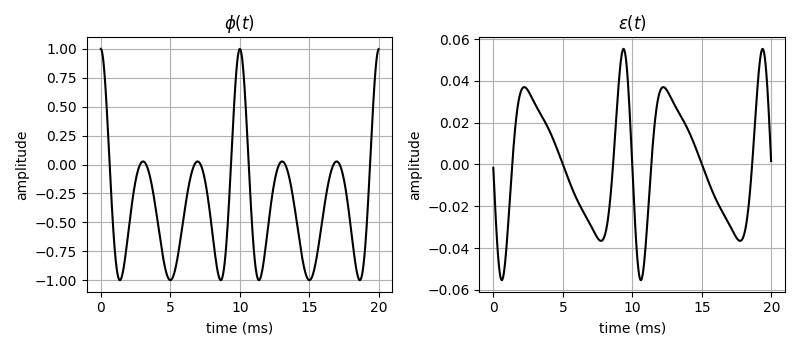
\includegraphics[width=0.8\columnwidth]{epsilon.png}
\caption{Modulation $\phi(t)$ (left) and error $\epsilon(t)$ (right) from Eq.~\ref{eq:eps},  with $f_{m_0} = f_{m_1} = 100$ Hz, $z_0=3$, and $f_s = 44.1$ KHz.}
\label{fig:epsilon}
\end{center}
\end{figure} 

\subsubsection{Second-order Error Analysis}

From Eqs.~\ref{eq:eps} and~\ref{eq:fmstacked}, the equation for second-order FM, as produced by a digital oscillator, 
becomes

\begin{equation}
\begin{split}
c(t) = \cos\Bigg( &  2\pi \int f_c  + z_1\left[f_{m_1} + z_0f_{m_0} \cos(2\pi f_{m_0}t)\right] \times \Bigg.\\
&\Bigg.\left[\cos(2\pi f_{m_1} t - z_0 [\sin(2\pi f_{m_0}t)]) + \epsilon(t)\right]dt\Bigg)
\end{split}.
\end{equation}
\smallskip

Translating this into a PM expression, we have

\begin{equation}
c(t) =  \cos\left(2\pi f_c t + z_1\sin(2\pi f_{m_1}  t + z_0 \sin(2\pi f_{m_0} t) + \theta(t)  \right),
\end{equation}
\smallskip

\noindent which excludes a low-amplitude term due to the carrier phase drift. Similarly to what we have observed in $\hat{\phi}(t)$, it does not contribute too much to the overall signal spectrum. The $\theta(t)$ function is therefore the significant differing factor between the ideal PM representation of second-order FM and its realisation with digital oscillators. It can be characterised as 
a slow phase modulation term that is dependent on the phase drift of the frequency-modulated oscillator,

\begin{equation}
\dot{\theta}(t)=  z_1[f_{m_1} + z_0 f_{m_0}\cos(2\pi f_{m_0} t)]\epsilon(t).
\end{equation} 
\smallskip

The nature of $\epsilon(t)$, and by consequence $\theta(t)$, is important. If the former contains any DC term,
the integration turns this into a linear modulation function, resulting in a low-frequency phase modulation
of the carrier wave. If there is no DC, then the errors are only responsible for a small fixed difference in the shape
of the FM signal in comparison to the corresponding PM formulation. 

Following these general ideas, we can proceed with a further analysis of the integration error signal.
The amplitude of $\epsilon(t)$ is inversely proportional to the sampling frequency; it is also proportional to the modulation frequency. The error signal $\epsilon(t)$ can be described as a phase-modulated carrier wave, and so we can predict that its components exist at $f_{m_1} \pm n f_{m_0}$ Hz. Therefore, if $f_{m_0} = f_{m_1}$, we should expect a DC term with a certain
amount of prominence in this signal, leading to low-frequency phase modulation artefacts, unless the phase of the DC component
can be made to be exactly $|\pi/2|$ (that is, an absolute sine phase). On the other hand, by setting $f_{m_0} = 2f_{m_1}$, we are able to suppress the slow phase modulation term (as no DC component is present in the FM signal), producing a steady output. 

\subsubsection{Mitigation}

In the case of stacked FM, the most adverse effects of digital integration errors have to do with the appearance of a low-frequency phase modulation term in the carrier wave. Furthermore, we may also observe these in feedback FM, where they can cause a small but perceived pitch detuning that is dependent on the feedback amount. These effects may be mitigated in four ways:\\

\begin{enumerate}
\item through limiting the $f_{m_n}: ... : f_{m_1} : f_{m_0}$ ratios to values where no sideband is present at 0 Hz;
\item by judiciously choosing a phase offset for $m_0(t)$ (etc) so that the spectrum of $\theta(t)$ does not
contain any energy, by forcing any 0 Hz sideband to be produced with a $|\pi/2|$ phase offset. This
modulator offset is a function of the modulation index $z_0$ (etc) and is independent of the modulation frequency.
\item computing a phase error signal that can be subtracted from $\nu(t)$.
\item employing an oversampling factor such as to minimise any integration errors.
\end{enumerate}
\bigskip

Of these, the first measure does not provide a general solution to the problem, it cannot be applied to feedback, 
and we are back more or less where we started. The second solution is more promising, such offsets can be computed for different configurations and stored in lookup tables. This may be a practical solution in cases where computing cost is at a premium.
The third method somehow defeats the purpose of the overall approach: if we have a good means of
generating a phase modulation signal, then employing FM does not seem to be ideal. However, it can be a good method
for error analysis, as demonstrated earlier in this section, rather than one used in deployment.

The final solution is probably the most practical; if we can approximate the continuous-time expression with a very fine degree of accuracy, we will not only be suppressing the integration errors, but we will also avoid any issues with foldover that may arise in the carrier wave spectrum (depending on the indices of modulation employed). It is often the case that FM/PM is prone to aliasing distortion; by oversampling, as is commonly done for instance with virtual analogue filters and oscillators \citep{VAreview}, we can solve these two issues at the same time. 

As an example, we can efficiently incorporate oversampling in the stacked FM code example shown earlier
using secret rabbit code~\citep{libsrc}, 

\begin{lstlisting}
class StackedFM {
  std::vector<double> table;
  Op<float> mod0; 
  Op<float> mod1;
  Op<float> car;
  std::vector<float> out;
  std::size_t ovs;
  SRC_STATE* stat;
  SRC_DATA cvt;
  
public:
  StackedFM(unsigned int fs,std::size_t os,
            std::size_t vsize = def_vsize) :
    table(1025),mod0(table,fs*os,vsize*os),
    mod1(table,fs*os,vsize*os),
    car(table,fs*os,vsize*os),
    out(vsize),ovs(os){
    int err;
    stat = src_new (SRC_SINC_FASTEST,1,&err);
    cvt.src_ratio = 1./ovs;
    cvt.input_frames = vsize*ovs;
    cvt.data_in = car.data();
    cvt.output_frames = vsize;
    cvt.data_out = out.data();
    cvt.end_of_input = 0;
    std::size_t n = 0;
    for(auto &s : table)
      s = std::cos(twopi/(table.size()-1)*n++);
  };

  ~StackedFM(){src_delete(stat);}

  unsigned int vsize(){return out.size();}
  unsigned int fs(){return car.sr()/ovs;}
  const float *data() {return out.data();}

  const std::vector<float> &operator()(float a,float fc,
                                       float fm0,float fm1,
				       float z0,float z1){
    mod0(z0,fm0);
    mod1(z1,fm1,mod0());
    car(a,fc,mod1());
    src_process(stat, &cvt);
    return out;
  }
};
\end{lstlisting}

In this C++ class, we may set the oversampling factor \lstinline{ovs} to achieve the 
mitigation effect described above depending on the original sampling rate used. In our tests, we have
experimentally observed that an oversampling factor of 4 is enough to reduce artefacts significantly.
Since these are related both to the sampling rate and the modulation frequencies applied, higher
modulation frequencies may require us to increase this oversampling factor. In systems where the
sampling rate is normally high, e.g. in the case of field programmable gate array (FPGA) oscillators, no oversampling is required and the methods described here find an optimal implementation platform.

\section{Conclusions}\label{sec:conclusions}

A simplistic approach to implementing second and higher-order FM arrangements has been shown to have limitations. Typical issues found in these situations are related to carrier drift, which is due to the presence of a DC component in a modulating waveform. Since the amount of energy at 0 Hz is defined by the index of modulation and is a function of the Bessel coefficient associated with the relevant sideband, any timbral changes in this case are accompanied by frequency glides that may be objectionable in practical applications. Such issues, caused by DC offsets in modulators, which also may pose practical limits to the use of feedback, are fully solved through the development of a PM-equivalent form of higher-order FM. Since higher-order PM is well understood and has been successfully applied in a variety of contexts, we propose that this may be a more suitable approach.

In this paper, we defined in good detail the differences between PM and FM, stemming from the fact that integration is directly present in the modulation of frequency. For this reason, to achieve a degree of control of higher-order modulation, there needs to be some care to ensure that these differences are dully respected. This means that it is not possible to solely employ the modulation signal to modify the frequency of the oscillator, but we also need to modulate its amplitude. From these
results, we then proposed a second-order FM arrangement that represents a PM-equivalent synthesis equation. From this formula we are then able to describe the resulting FM spectrum by employing a similar approach to the derivation of the complex PM spectrum. 

Higher-order modulation topologies can then be implemented as an extension of the second-order approach. 
For these, we found that an operator approach may be helpful. We have then put forward the basic design of such a black box, demonstrating its equivalence to the second-order design shown earlier. With these, it is possible to freely construct various FM topologies, including feedback FM, as it is customarily done with PM. We completed the discussion with a full reference implementation of operator-based FM.

While it was beyond the scope of this article to consider in detail possible applications of higher-order FM synthesis, we may cite a few. Generally, the technique is useful in situations where it is not convenient or practical to modulate the phase of a signal. One such example is the case of the synthesis methods employed in the Summit synthesiser oscillator implementation \citep{Summit}. Although these have not been published and it is not possible to exactly determine their details, it is a reasonable assumption that PM is either not possible or not ideal since they opted to implement FM in a somewhat na\"{i}ve form (as per our earlier analysis). Another application may be found in analogue signal processing, where it is often the case that (linear) FM can be employed directly, whereas PM poses more difficulties \citep{LazzariniTimoney2021}. Thus a simplification in circuit design may be also another factor that would favour the use of the technique.

Within a digital signal processing environment, however, we have noted that there are a few practical issues arising within
the scenarios of stacked and feedback FM introduced here. These have to do with numerical errors arising 
from the discrete nature of the integration filter employed in the implementation of an oscillator. In the case of a modulation stack, we have observed that such errors result in a phase modulation term that is not present in the
continuous-time analysis of Section \ref{sec:theory}. This can introduce periodic modulation artefacts in the carrier signal that may be objectionable. In the case of Feedback FM, the errors insert an extraneous DC term in the signal that has an obvious, although small, effect on pitch. We provided an analysis of these errors, their effects, and possible mitigation. We realise that these issues may 
result in the methods described here to be of limited application to users in a typical 
desktop computing environment. However for developers in specialist digital platforms
modulation, and practitioners of analogue synthesis may find benefit from the theory of higher-order FM.
In some applications, such as the extremely high sampling rate oscillator implementations (e.g. using FPGA hardware, as in the case of Summit synthesiser, running in the two-digit MHz range), these digital
signal processing issues may not be of concern.

Code examples and scripts used for the signal analysis in this paper can be found at\\

\begin{center}
\url{https://github.com/vlazzarini/highorderfm}
\end{center}

\bibliography{paper}
\bibliographystyle{apacite}


\end{document}